% !TEX root = ../main.tex
\chapter{Introduction}
\label{chapter:Introduction}


\section{Motivation}

A worthwhile use of the vast computational resources available in 2018 is on seismic simulations. 

\begin{description}
	\item[SeisSol]
    Simulates earthquakes, specifically, dynamic rupture processes and seismic wave propagation over an unstructured tetrahedral mesh. 

    \item[ADER-DG]
    A numerical method which uses Discontinuous Galerkin discretization in space and ADER discretization in time. It avoids a global system matrix, using local element matrix operations instead.

    \item[Small Sparse Matrix Multiplications]
    The compute kernels resemble the operation shown below, applied recursively. Different sparsity patterns are used, but they are all known at compile time.
\end{description}

\begin{figure}
  \centering
  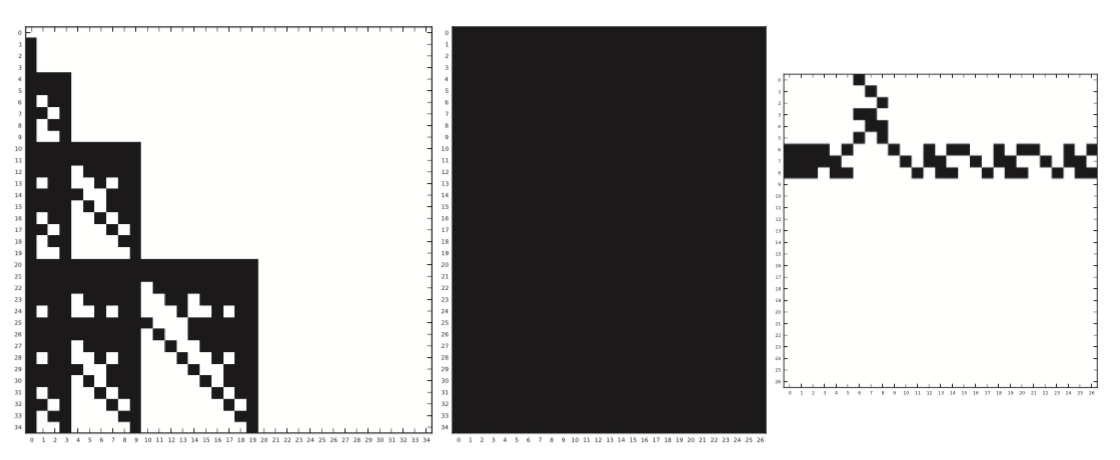
\includegraphics[height=3cm]{images/seissol_visc.png}
  \caption{Common sparsity patterns in SeisSol}
  \label{fig:seissol_star}
\end{figure}

\section{Hardware constraints}
\label{section:knl}

Although the motivation is straightforward, it is challenging in practice because the problem is working against current trends in computer architecture. A growing number of the Top500 computers are using manycore processors such as GPUs or Xeon Phis. This trend is likely to continue because it allows greater parallelism and throughput at a lower energy cost. For this particular work, the goal is further optimize the kernels for LRZ's CoolMUC3 cluster, which uses Knights Landing.

Knights Landing (KNL) is the second-generation Intel Xeon Phi, a manycore processor that offers greater parallelism and less power consumption in exchange for a slower clock speed. An overview is given by~\cite{Sodani:2016:KLS:2927511.2927563} and a more comprehensive resource is given by~\cite{Jeffers:2016:IXP:3050856}. Unlike its predecessor, Knights Corner, KNL is a host processor rather than a coprocessor, which means that it can run the entire x86-64 instruction set, albeit with a performance penalty for some operations. KNL has two kinds of memory, a high-bandwidth MCDRAM and a high-capacity DDR4. Each processor contains between 64 and 72 cores with 4 hyperthreads per core, resulting in at least 256 logical CPUs. The instruction-level parallelism is similarly impressive due to the AVX-512 instruction set extensions. These provide 32 vector registers, each of which holds 64 bytes, allowing 8 double-precision floating point numbers to be operated on simultaneously in each \gls{VPU}. Instruction-level performance is further improved by an enhanced \gls{FMA} instruction, which performs $c := c + a*b$ in a single cycle, optionally including a broadcast and a mask. Thus the theoretical peak performance is given as:

\[
2~\frac{\text{VPUs}}{\text{core}} \times 16~\frac{\text{double flops}}{\text{VPU} \cdot \text{cycle}} \times 1.3~\frac{\text{GCycles}}{\text{sec}} = 41.6~\frac{\text{double GFlop}}{\text{sec}\cdot \text{core}}
  \label{eq:knl_peak_perf}
\]

\[
36~\frac{\text{tiles}}{\text{chip}} \times 2~\frac{\text{cores}}{\text{tile}} \times 41.6~\frac{\text{double~GFlop}}{\text{sec}\cdot \text{core}} = 3.0~\frac{\text{double TFlop}}{\text{sec}\cdot \text{chip}}
  \label{eq:knl_peak_perf}
\]

This peak performance is in practice merely an upper bound, as it assumes a steady-state throughput of 2 FMAs per cycle. The algorithms which approach this are mainly dense matrix multiplication or LU/Cholesky factorization. If the algorithm cannot be vectorized at all, the attainable performance drops by a factor of 8, and if it cannot use the FMA instructions, it drops by a further factor of 2. Hence inherently scalar algorithms perform dramatically worse. This may be a reasonable tradeoff: since scalar algorithms are much more likely to be memory-bound, the extra flops might be wasted. Nevertheless this provides a strong incentive to find creative ways to make the most of the vector registers. 

Another key constraint is cache bandwidth. With only one store unit, KNL can store at most 64B/cycle, corresponding to one vector register. This means that it is essential to accumulate all possible changes to that vector register before storing it. It also makes loop unrolling quite important for amortizing the cost of loads and stores.

A number of related bottlenecks encompass the instruction pipeline. Because Knights Landing was derived from the older Silvermont architecture, which was optimized for low power consumption, the instruction pipeline is simpler and narrower. The instruction cache provides 16B/cycle, and the decoder handles 2 instructions/cycle. For comparison, a single \gls{FMA} instruction takes up between 7 and 10 bytes. The least expected constraint, however, is that the out-of-order execution pipeline can only issue 2 instructions per cycle. This means that any instruction which is not vector arithmetic (e.g. an FMA) \emph{displaces} a vector arithmetic instruction, halving the potential computational efficiency of one cycle.

In summary, there is a variety of architectural constraints which make Knights Landing well-suited for large dense operations, and correspondingly less well-suited for small sparse operations. SeisSol still performs well on KNL, because of its scalability across threads and nodes. Nevertheless its performance responds to optimizations of its inner matrix kernels.

\begin{figure}[tb]
\centering
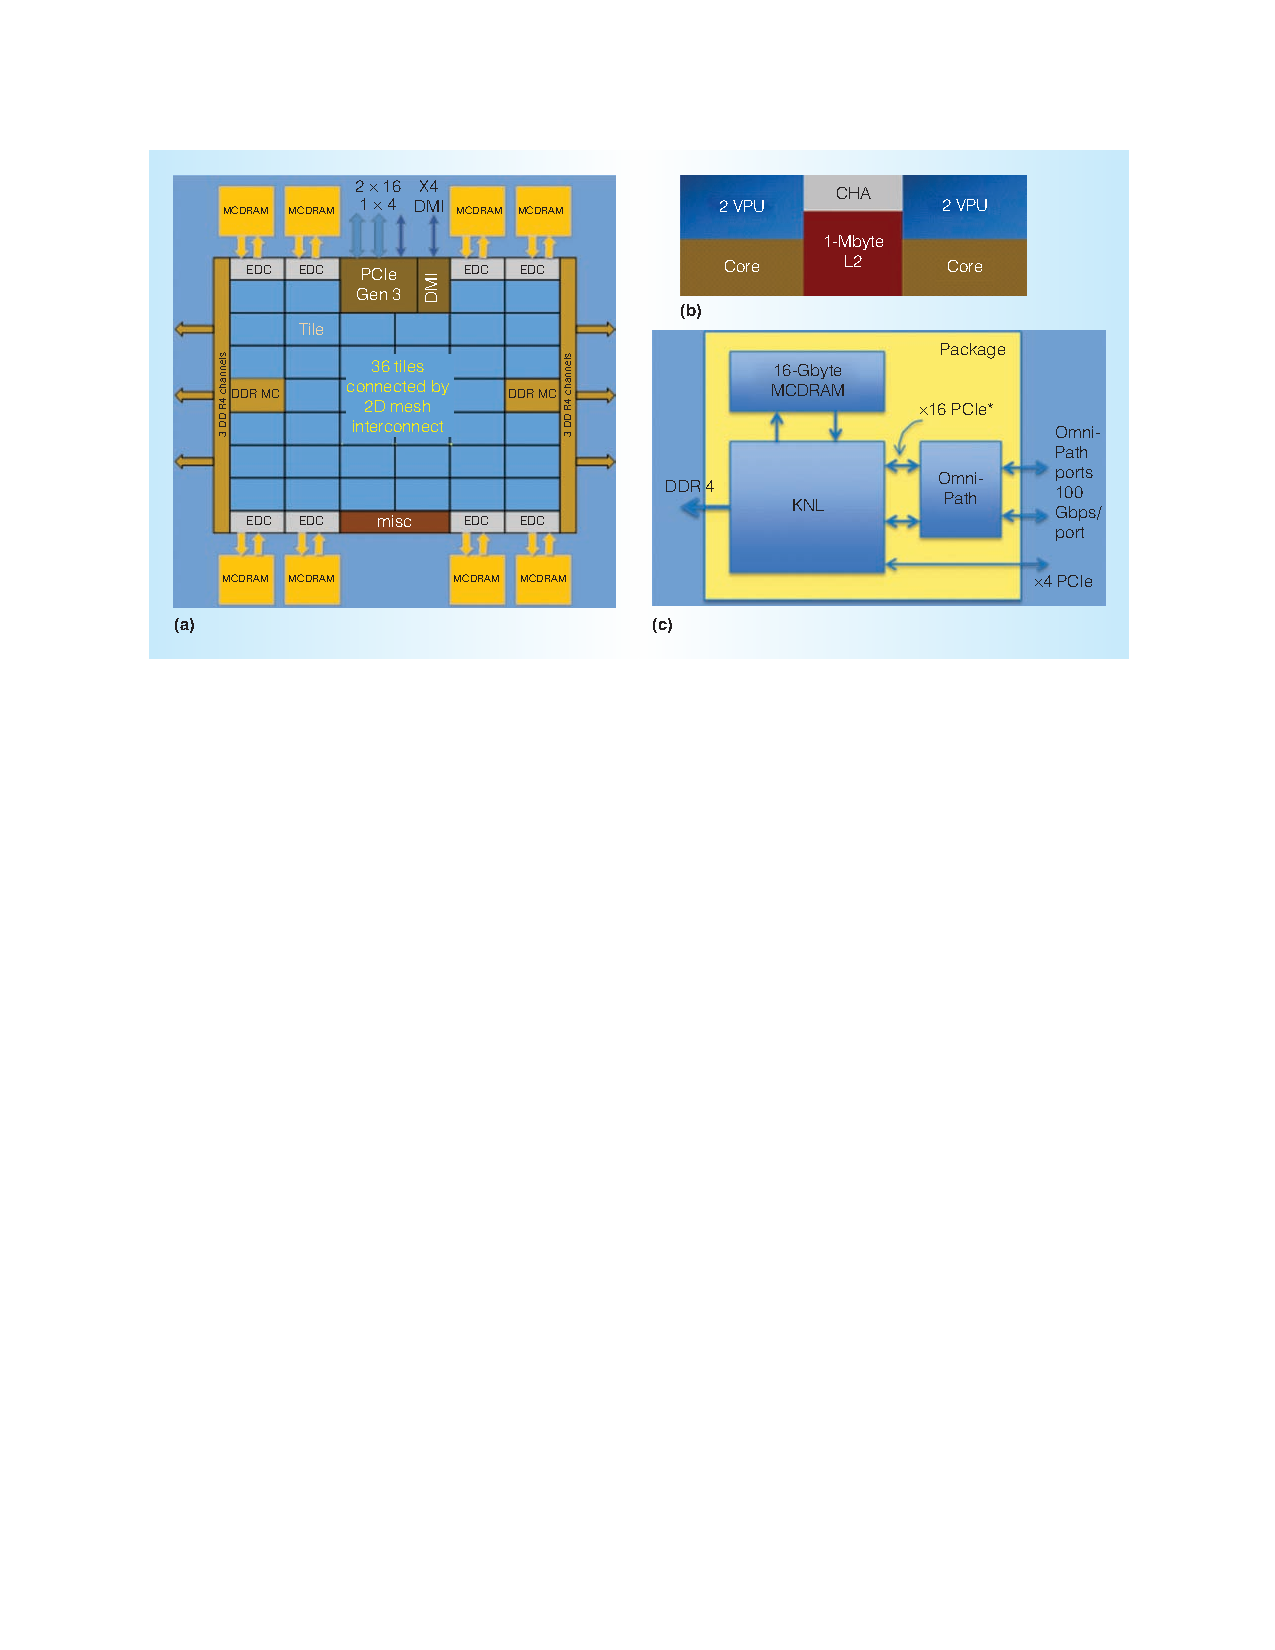
\includegraphics[width=\textwidth]{images/knl_arch.pdf}
\caption{Block diagram of the Knights Landing architecture, taken from~\cite{Sodani:2016:KLS:2927511.2927563}. As shown in (a), each processor is divided into 36 tiles connected in a 2D mesh. As shown in (b), each tile contains 2 cores and a shared L2 cache. Each core has two VPUs and its own L1 caches.}
\end{figure}


\section{Previous approaches}

    Significant work has already been undertaken to optimize the performance of the sparse matrix kernels. There are three main approaches which have been explored. Originally an off-the-shelf sparse matrix routine was used. Later, this was replaced by a custom kernel generated for each specific sparsity pattern, introduced by Breuer in~\cite{breuer}. Finally, this was replaced by a dense kernel optimized for small matrices and wide registers, introduced by Heinecke in~\cite{Heinecke:2016:LAS:3014904.3015017}. The decision to use the dense kernel on KNL is discussed in depth in~\cite{Jeffers:2016:IXP:3050856}. 
    
    There are several properties of the SeisSol matrix chains which can be leveraged to improve performance. Firstly, these matrices remain quite small: the largest matrix dimension under consideration is 56 and the smallest is 9. This means that they can be assumed to fit in cache. Secondly, the sparsity patterns are constant. This is because they are derived from the basis functions, which themselves depend on the desired order of accuracy and the choice of viscous damping model. These properties do not appear to play to the strengths of Knights Landing, but they do provide the programmer something to work with.

    There are also several constraints. SeisSol is already carefully parallelized via MPI and OpenMP, and the kernels are expected to run within each thread. This means that only instruction-level parallelism shall be considered in this work. Likewise, the strategy for utilizing KNL's high-bandwidth memory is determined at a much higher level, and shall not be considered here.

\subsection{Off-the-shelf sparse matrix routines}

      The most straightforward approach to handling SeisSol's small sparse matrix kernels is to use off-the-shelf dense-by-sparse multiplication routines such as those provided by MKL~\cite{IntelCSCMM}. This approach benefits from being very general: it places no constraints on the matrix size or sparsity, and relegates knowledge of the sparsity pattern to runtime. The matrix is stored in a common format such as CSC, which store indexes so that no information is lost and other routines may interact in a relatively abstract manner. The routines themselves take up a small, fixed amount of memory which does not depend on the matrix sparsity pattern.

      However, Breuer and Heinecke~\cite{breuer} show that this approach leaves a considerable amount of performance on the table. Firstly, they have a high memory usage. Secondly, they have a low computational intensity. Thirdly, they are difficult to vectorize because . Finally, the innermost loop over the entries of the sparse matrix cannot be unrolled, because it relies on control flow. Due to the issue width constraint, 

      \begin{description}
        \item[Cache bandwidth] The indexes 
        \item[Computational intensity]
        \item[Inability to unroll the innermost loop] This hurts pipeline efficiency.
        \item[Scalar operations]

        The indices are looked up at runtime. Firstly, this requires storing the indices, doubling the amount of memory needed. If only one matrix is sparse, the total number of flops is $2 * m * n * nnz$, with nnz=1/4*n*k, this means that the arithmetic intensity [FLOPs/byte] is 1/8 that of dense matrix multiplication. 
        Although the format lays everything out in memory as efficiently, the algorithm must nevertheless loop over k. The resulting control dependency prevents . The fact that the sparsity pattern is only known at compile time prevents unrolling. 
        A dense-by-sparse algorithm would still benefit from vectorization, but if the 

      \end{description}


      Standard compressed-sparse-column multiplication
        \begin{itemize}
          \item[$+$] Algorithm uses a (small) constant number of instructions.
          \item[$-$] Index lookups require indirect memory access, causing lots of problems for the execution pipeline.
          \item[$-$] $sparse \times sparse$ is fundamentally scalar. (However, BSR can be vectorized.)
          \item[$-$] Disregards the fact that the sparsity pattern is known at compile time.
        \end{itemize}




\subsection{Sparse kernel generation}
    
      Breuer's solution to the inefficiencies in the previous approach was to generate a custom kernel for each sparse matrix product. The generator runs in a separate phase before compilation, and takes as inputs the matrix sizes, the target architecture, and a file describing the sparsity pattern. From this information it emits a C function to perform the multiplication. These functions differ from their predecessors in several key ways. 

      \begin{enumerate}
        \item The sparsity pattern is expressed in a direct sequence of multiply-adds; indices are hardcoded. This means that the indirect lookups are eliminated completely, and the indices need not even be present. Thus the CSC format becomes a `virtual' CSC format, effectively just an array of nonzero matrix entries ordered by columns. This in turn takes pressure off the caches. 

        \item The code has far less control flow. Whereas the classic kernels must loop over individual elements of B, these kernels have in effect unrolled both inner loops, so that only the outermost loop remains. The compiler is instructed to vectorize this. 

        \item This unrolling emits one FMA per nonzero in the matrix B, which means that the size of this algorithm can run up against the instruction cache limit if B becomes too large or dense.

        \item The generator for CSC dense-by-sparse is dramatically simpler and more performant than for CSC sparse-by-dense. This asymmetry comes from the vectorization, and will be discussed in more detail in Section~\ref{section:asymmetry}.

      \end{enumerate}

      This approach yielded a speedup of 2.2 on Sandy Bridge using AVX-128 instructions. However, the performance declined on Haswell and Knights Landing. 

      The following justification for switching to dense is quoted straight from~\cite{Jeffers:2016:IXP:3050856}:
      \begin{quotation}
      As we are operating out of L1 without significant reuse in the case of the sparse variant, this limits us to at most 50\% of peak performance of the core as we can only store one register per cycle. The dense variants have register accumulators and can therefore exploit both VPUs and catch up.
      \end{quotation}

      This is an algorithmic limitation, not an architectural one. If the code generator scheduled its loads, stores, and FMAs such that accumulated into a carefully-sized block of C, the 



\subsection{Dense kernel generation}

    The dense kernel generation is part of a separate library called libxsmm.~\cite{Heinecke:2016:LAS:3014904.3015017} Libxsmm 

    \begin{itemize}
      \item Memory access patterns and register blockings optimized for KNL

      \item (Implementation) Code generator emits assembly directly 

      \item Filling in zero entries wastes both flops and memory bandwidth

    \end{itemize}




  \section{Goals, approach, and design space}

  Each of the existing algorithms discussed in the preceding section encounter different bottlenecks and constraints. \py{SpGemm} and \py{libxsmm} solve a more general problem than strictly necessary, and Breuer does not use registers Thus there appears to be room to create more complicated algorithms which combine the desirable features of each. The three existing algorithms can be thought of as poles in a barycentric design space, and the aim is to find points in the middle which finesse around the bottlenecks in the corners. One corner has high compute intensity and an optimal register blocking, but wasted flops; another has no wasted flops but many control dependencies and lower compute intensity; the last has no wasted flops and high compute intensity, but no register blocking. The center ought to have decent compute intensity, a decent register blocking, few control dependencies, and few wasted flops. 


  To keep the scope of this work bounded, we adhere to following assumptions:
  \begin{itemize}
    \item The sparse matrix has a fixed pattern which is known at compile time.
    \item The memory layout of the sparse matrix is not constrained elsewhere.
    \item All matrices fit in the L2 cache: $(mn + mk + kn)\cdot 8 \leq 1e6$
  \end{itemize}

  Within this framework, we consider variations of the following:
  \begin{itemize}
    \item Modifications of the sparsity pattern
    \item Modifications of the control flow
    \item The memory layout of the sparse matrix
    \item The block sizes, if a block decomposition is used
    \item The ordering and unrolling of the loop nest
  \end{itemize}


Although interesting, we disregard prefetching, instruction alignment, and register assignment. 

The goal of this work is to find algorithms which might outperform the status quo, and write a code generator which will emit an instance of each relevant algorithm for a given problem. The generator should be able to handle different matrix sizes, number of nonzeros, and sparsity patterns, while staying within the aforementioned assumptions. 

Once implemented, the generators can be tested -- using the actual SeisSol matrices -- to determine if they yield a speedup. Equally interesting is exploring the algorithm's problem space constraints. Using both the observed and estimated performance, we can address the questions ``which problems can this algorithm handle efficiently?'' and ``which algorithm is best for a given problem?''. 

Each algorithm requires additional tuning parameters, and the effect of these should also be estimated and tested, addressing the question ``which parameters yield the best kernel for a given problem?''. If possible, heuristics should be given in order to choose these parameters automatically.

   
\section{Roadmap} 
  This work is broken down as follows. Chapter 2 lays out the fundamental concepts and terminology. Chapter 3 covers a progression of different dense-by-sparse kernels in depth, and discusses strategies for sparse-by-dense and tensor kernels which might benefit from a similar treatment. Chapter 4 discusses the design of the code generator, and provides a brief manual illustrating its use. Chapter 5 walks through some experiment results, attempting to discern performance and scaling characteristics. Finally, Chapter 6 wraps everything up.










